\chapter{От локального сохранения к уравнениям поля Эйнштейна}

Уравнения поля Эйнштейна достаточно просты, чтобы записать их в одну строку, и печально известны тем, насколько неприятно раскрывать их по компонентам. У метрики много символов Кристоффеля; символы Кристоффеля содержат производные метрики; а тензор кривизны содержит и производные, и произведения символов Кристоффеля. Еще до попытки что-либо решить вычисления могут занимать страницы. Для конкретной метрики разумным способом справиться с этой бухгалтерией часто оказываются системы символьных вычислений.

Сами принципы гораздо яснее, чем вычисления. Поэтому мы не будем начинать с покомпонентного разбора уравнений. Мы спросим, какого рода уравнение требуется для гравитации. Рассуждение начинается с ньютоновской теории, проходит через локальное сохранение и завершается обнаружением той единственной комбинации тензоров кривизны, которую можно непротиворечиво приравнять потоку и плотности энергии и импульса. Во всей главе мы используем \(c=1\).

\section{Ньютоновская улица с двусторонним движением}

В гравитации действуют два взаимодополняющих предписания. Гравитационное поле указывает материи, как двигаться, а материя указывает гравитационному полю, каким ему быть. Эта двусторонняя связь уже видна в ньютоновской механике.

Пусть \(\phi(\mathbf{x},t)\) — ньютоновский гравитационный потенциал. Пробное тело массы \(m\) испытывает силу
\begin{equation}
 \mathbf{F}=-m\nabla\phi.
\end{equation}
Совмещая это с \(\mathbf{F}=m\mathbf{a}\), мы сокращаем пробную массу:
\begin{equation}
 \mathbf{a}=-\nabla\phi.
\end{equation}
Это первое направление такого двустороннего движения. Когда поле задано, оно определяет, с каким ускорением будет двигаться любое свободно падающее тело, независимо от массы этого тела.

Обратное направление задается уравнением Пуассона,
\begin{equation}
 \nabla^2\phi=4\pi G\rho,
 \qquad
 \nabla^2=
 \frac{\partial^2}{\partial x^2}
 +\frac{\partial^2}{\partial y^2}
 +\frac{\partial^2}{\partial z^2},
 \label{eq:poisson}
\end{equation}
где \(\rho(\mathbf{x},t)\) — масса на единицу объема. Коэффициент \(4\pi\) можно было бы перенести в определение \(G\), но тогда он просто появился бы в другом месте. Уравнение~\eqref{eq:poisson} утверждает, что распределение материи является источником потенциала.

Для сферически симметричного тела полной массы \(M\) внешнее решение имеет вид
\begin{equation}
 \phi(r)=-\frac{GM}{r}.
 \label{eq:newton-potential}
\end{equation}
Плотность может быть сосредоточена вблизи центра, распределена равномерно или плавно спадать к поверхности. Для внешнего решения важны только сферическая симметрия и полная масса. Вне вещества \(\nabla^2\phi=0\); дифференцирование \(1/r\) затем дает силу, обратно пропорциональную квадрату расстояния. Если нас интересует только внешняя область, мы можем стянуть источник в точку и использовать то же выражение всюду, кроме этой точки.

\begin{classroomqa}
\audiencequestion{Должна ли плотность внутри сферического тела быть постоянной, а затем на его границе скачком переходить в нуль?}
\lecturerresponse{Нет. Для этого рассуждения она должна быть сферически симметричной, но не обязана быть постоянной и не обязана испытывать скачок. Она может плавно убывать до нуля. Ни одна из этих внутренних деталей не меняет внешний потенциал, который зависит только от полной массы.
\lecturetimestamp{00:09:13--00:09:37}}
\end{classroomqa}

Эта полевая формулировка выглядит более локальной, чем прямая сила между удаленными массами, но ньютоновская гравитация все еще содержит мгновенное действие на расстоянии. Переместите источник, и ньютоновский потенциал сразу изменится повсюду. Общая теория относительности должна заменить и этот мгновенный отклик, и сам закон силы.

\section{Слабополевой намек, но еще не уравнение}

Релятивистская версия первого предписания уже известна: как только задана метрика пространства-времени, свободно падающие частицы следуют по геодезическим пространства-времени. Теперь нам нужна релятивистская замена уравнения Пуассона — предписание, посредством которого материя определяет метрику.

Геометрия Шварцшильда дает подсказку. Ее временная-временная компонента равна
\begin{equation}
 g_{00}=1-\frac{2GM}{r}.
\end{equation}
Используя уравнение~\eqref{eq:newton-potential}, получаем
\begin{equation}
 g_{00}=1+2\phi.
\end{equation}
Следовательно,
\begin{equation}
 \nabla^2g_{00}=2\nabla^2\phi=8\pi G\rho.
 \label{eq:weak-mnemonic}
\end{equation}

К уравнению~\eqref{eq:weak-mnemonic} следует относиться с осторожностью. Это мнемоническая формула, а не уравнение Эйнштейна. В нем используется выделенная компонента метрики и нерелятивистский источник. Тем не менее оно показывает ту структуру, которую мы ищем: плотность материи по одну сторону и вторые производные геометрии по другую. Это грубый мост от уравнения Пуассона к ковариантному полевому уравнению.

Правая часть теперь требует более пристального внимания. В релятивистских единицах масса есть энергия, поэтому \(\rho\) прежде всего следует понимать как плотность энергии. Но плотность энергии — не полный релятивистский объект. Чтобы увидеть, что ее сопровождает, начнем с более простой сохраняющейся величины.

\section{Плотность заряда, ток и локальный закон сохранения}

Пусть \(Q\) — электрический заряд, а \(\sigma\) обозначает плотность заряда:
\begin{equation}
 \sigma=\lim_{\Delta V\to0}\frac{\Delta Q}{\Delta V}.
\end{equation}
Плотность отвечает на вопрос, сколько заряда содержится в малом пространственном объеме в данный момент. Ток задает другой вопрос. Поместите в пространстве бесконечно малую ориентированную площадку и посчитайте, сколько заряда проходит через нее на единицу площади за единицу времени. Три возможные ориентации дают пространственные компоненты тока \(J^i\).

Размерностное сравнение поучительно. Плотность заряда — это заряд, деленный на произведение трех пространственных длин. Ток — это заряд, деленный на произведение двух пространственных длин и одного интервала времени. Когда \(c=1\), время и длина имеют одинаковые единицы, так что плотность и ток имеют одну и ту же размерность. Они объединяются в четырехвектор:
\begin{equation}
 J^\mu=(J^0,J^1,J^2,J^3),
 \qquad J^0=\sigma.
\end{equation}

Закон сохранения заряда — это не просто утверждение о том, что полный заряд во Вселенной остается постоянным. Он локален. Заряд не может исчезнуть в аудитории и мгновенно появиться у Альфы Центавра. Если он покидает область, то должен пересечь ее границу. Для малого ящика убывание заряда внутри равно потоку наружу через его стенки. Теорема Гаусса дает
\begin{equation}
 \dot{\sigma}+\nabla\cdot\mathbf{J}=0,
\end{equation}
или, используя соглашение суммирования,
\begin{equation}
 \partial_\mu J^\mu=0.
 \label{eq:charge-continuity}
\end{equation}
В криволинейных координатах соответствующее тензорное уравнение записывается с ковариантной производной:
\begin{equation}
 D_\mu J^\mu=0.
\end{equation}
Назначение ковариантной производной не декоративно. Она делает это утверждение осмысленным в любой системе координат.

\section{Почему энергии и импульсу нужны два индекса}

Сам заряд инвариантен. Наблюдатели, движущиеся относительно друг друга, согласны относительно заряда электрона, хотя они не согласны относительно плотности заряда или тока. Движущийся наблюдатель видит лоренц-сокращенные объемы и может видеть поток зарядов там, где другой наблюдатель видит покоящиеся заряды. Поэтому при смене системы отсчета плотность и ток смешиваются, хотя полный заряд — нет.

С энергией и импульсом дело обстоит сложнее. Даже их полные значения зависят от системы отсчета. Один наблюдатель может видеть частицу покоящейся, несущей только свою энергию покоя и не имеющей пространственного импульса. Другой наблюдатель, проходящий мимо, видит и кинетическую энергию, и импульс. Эти четыре величины образуют четырехвектор импульса
\begin{equation}
 P^\nu=(P^0,P^1,P^2,P^3),
 \qquad P^0=E.
\end{equation}
Каждая компонента \(P^\nu\) локально сохраняется. Поэтому каждая имеет и плотность, и поток. Один индекс указывает сохраняющуюся величину; второй индекс указывает плотность или направление потока.

Начнем с энергии. Ее плотность равна \(T^{00}\). Энергия тоже может проходить через площадку, поэтому \(T^{0i}\) — это поток энергии в направлении \(x^i\). Теперь возьмем \(i\)-ю компоненту импульса. Ее плотность равна \(T^{i0}\), а ее поток в направлении \(x^j\) равен \(T^{ij}\). В этом соглашении:
\begin{itemize}
 \item \(T^{00}\) — плотность энергии;
 \item \(T^{0i}\) — поток энергии в направлении \(i\);
 \item \(T^{i0}\) — плотность \(i\)-й компоненты импульса;
 \item \(T^{ij}\) — поток \(i\)-й компоненты импульса через поверхность, нормаль к которой направлена вдоль \(j\).
\end{itemize}
Пространственный блок \(T^{ij}\) позже будет распознан как напряжения: его диагональные элементы включают давления, а внедиагональные описывают сдвиг.

\begin{classroomqa}
\audiencequestion{Если \(T^{m0}(x)\) называют плотностью \(m\)-й компоненты импульса, означает ли \(x\) само по себе \(m\)-ю компоненту положения?}
\lecturerresponse{Нет. Аргумент \(x\) обозначает точку пространства-времени, в которой вычисляется плотность; он представляет все координаты. Индекс \(m\) указывает, какая компонента импульса подсчитывается.
\lecturetimestamp{00:41:07--00:41:27}}
\end{classroomqa}

Для каждого фиксированного \(\nu\) локальный закон сохранения дает уравнение непрерывности:
\begin{equation}
 D_\mu T^{\nu\mu}=0.
 \label{eq:stress-continuity}
\end{equation}
Четыре значения \(\nu\) дают одно уравнение для энергии и три — для импульса. Вместе плотности и потоки образуют тензор энергии-импульса.

\begin{figure}[htbp]
\centering
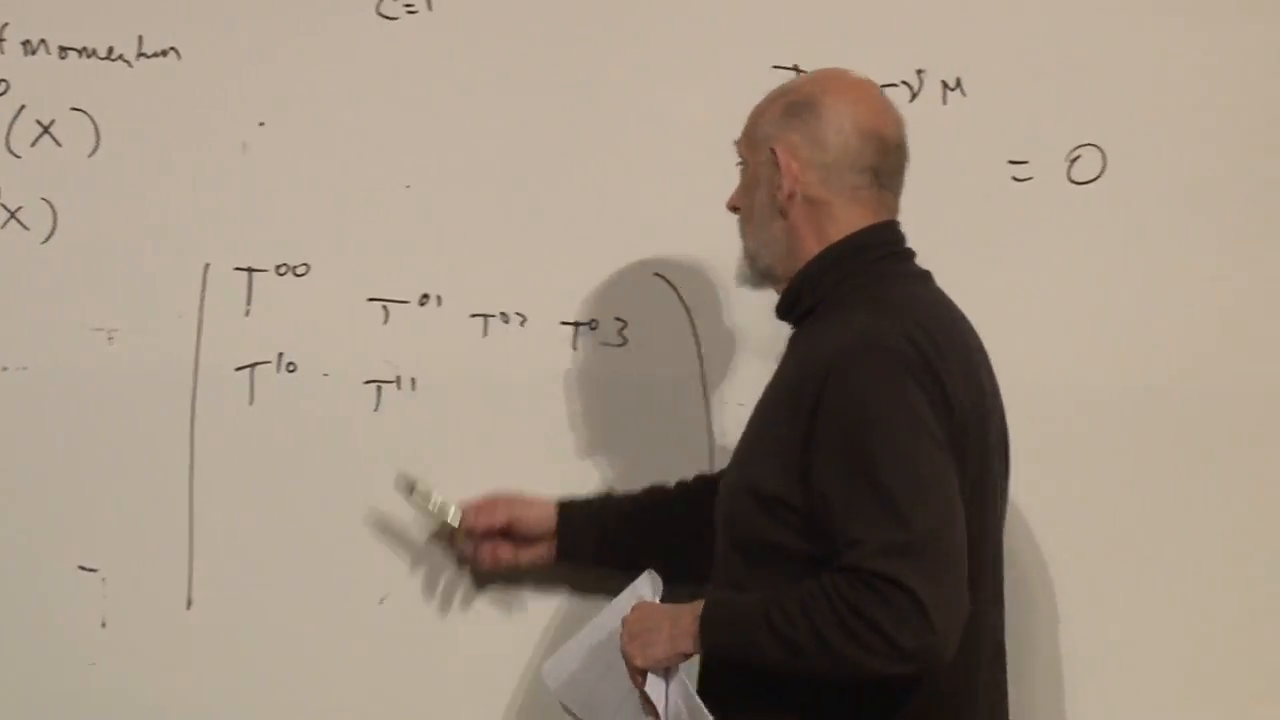
\includegraphics[width=0.84\textwidth]{lecture_09_figure_02.png}
\caption{Формирующийся на доске массив энергии-импульса. Первый индекс выбирает энергию или компоненту импульса; второй выбирает плотность или поток.}
\lectureframe{00:44:30}
\end{figure}

Полный массив имеет вид
\begin{equation}
 T^{\mu\nu}=
 \begin{pmatrix}
 T^{00}&T^{01}&T^{02}&T^{03}\\
 T^{10}&T^{11}&T^{12}&T^{13}\\
 T^{20}&T^{21}&T^{22}&T^{23}\\
 T^{30}&T^{31}&T^{32}&T^{33}
 \end{pmatrix}.
\end{equation}
Еще одна теорема релятивистской механики и теории поля утверждает, что важный для гравитации тензор энергии-импульса симметричен:
\begin{equation}
 T^{\mu\nu}=T^{\nu\mu}.
 \label{eq:stress-symmetry}
\end{equation}
В частности, поток энергии и плотность импульса — это соответствующие внедиагональные элементы, рассматриваемые с противоположных сторон. Симметрия также позволяет записать уравнение~\eqref{eq:stress-continuity} в привычной форме
\begin{equation}
 D_\mu T^{\mu\nu}=0.
 \label{eq:stress-conservation}
\end{equation}

\begin{classroomqa}
\audiencequestion{Почему у энергии-импульса появился дополнительный индекс, тогда как току заряда требовался только один?}
\lecturerresponse{Индекс тока уже различает плотность и направление потока. Заряду не нужна дополнительная метка, потому что сохраняющийся заряд — скаляр. Энергия и три компоненты импульса сами образуют четыре компоненты, поэтому первый индекс указывает, какая сохраняющаяся величина имеется в виду, а второй — идет ли речь о плотности или о потоке.
\lecturetimestamp{00:45:31--00:47:24}}
\end{classroomqa}

\begin{classroomqa}
\audiencequestion{Симметрична ли вся матрица \(T^{\mu\nu}\), а не только элементы потока энергии и плотности импульса?}
\lecturerresponse{Да. Симметрична вся матрица. Подробный смысл ее пространственных элементов, включая давление и напряжения, будет разобран позже.
\lecturetimestamp{00:47:32--00:47:54}}
\end{classroomqa}

Таким образом, плотность энергии была лишь одним угловым элементом более крупного объекта. Источником гравитации не может непротиворечиво быть одно лишь \(T^{00}\); должен входить полный тензор.

\section{Закон не может выделять одну компоненту}

Необходимость тензорного уравнения видна и без каких-либо вычислений кривизны. Пусть \(A_i\) и \(B_i\) — векторы, а предлагаемый закон утверждает только \(A_3=B_3\). Если это равенство должно выполняться в любой повернутой системе отсчета, повернем третью ось во вторую. Тогда тот же закон утверждает \(A_2=B_2\); еще один поворот дает \(A_1=B_1\). На самом деле закон, не зависящий от системы отсчета, представляет собой векторное уравнение
\begin{equation}
 A_i=B_i.
\end{equation}

Преобразования Лоренца распространяют тот же довод и на время. Если \(A^0=B^0\) должно выполняться в любой инерциальной системе отсчета, бусты смешивают временную компоненту с пространственными и вынуждают полное уравнение \(A^\mu=B^\mu\). Хорошие релятивистские законы должны приравнивать тензоры одного и того же типа.

Ньютоновское мнемоническое правило выделяло \(T^{00}\), но релятивистское уравнение должно иметь вид
\begin{equation}
 G_{\mu\nu}=8\pi G\,T_{\mu\nu},
 \label{eq:field-schematic}
\end{equation}
где символ \(G_{\mu\nu}\) поначалу — лишь условное обозначение. Теперь ясны его необходимые свойства:
\begin{enumerate}
 \item он должен быть симметричным тензором второго ранга;
 \item он должен быть построен из метрики, а не из материи;
 \item в нем должны содержаться две производные метрики;
 \item его ковариантная дивергенция должна обращаться в нуль.
\end{enumerate}
Последнее условие следует из уравнения~\eqref{eq:stress-conservation}.

\section{Поиск среди тензоров кривизны}

Символы Кристоффеля содержат одну производную метрики:
\begin{equation}
 \Gamma^\sigma_{\tau\nu}
 =
 \frac12 g^{\sigma\delta}
 \left(
 \partial_\tau g_{\delta\nu}
 +\partial_\nu g_{\delta\tau}
 -\partial_\delta g_{\tau\nu}
 \right).
 \label{eq:christoffel}
\end{equation}
Они не являются тензорами, поэтому сами по себе не могут дать левую часть. Тензор кривизны Римана является тензором:
\begin{equation}
 R^\rho{}_{\sigma\mu\nu}
 =
 \partial_\mu\Gamma^\rho_{\nu\sigma}
 -\partial_\nu\Gamma^\rho_{\mu\sigma}
 +\Gamma^\rho_{\mu\lambda}\Gamma^\lambda_{\nu\sigma}
 -\Gamma^\rho_{\nu\lambda}\Gamma^\lambda_{\mu\sigma}.
 \label{eq:riemann}
\end{equation}
Его первые два члена содержат вторые производные метрики; последние два содержат произведения первых производных. Это в точности тот дифференциальный порядок, на который указывало ньютоновское уравнение.

Трудность состоит в структуре индексов. \(R^\rho{}_{\sigma\mu\nu}\) имеет четыре индекса, тогда как \(T_{\mu\nu}\) — два. Свертка подходящей пары верхнего и нижнего индексов дает тензор Риччи,
\begin{equation}
 R_{\mu\nu}=R^\lambda{}_{\mu\lambda\nu}.
 \label{eq:ricci}
\end{equation}
Другие на первый взгляд возможные свертки либо обращаются в нуль из-за симметрий тензора Римана, либо воспроизводят тот же объект с точностью до знака и соглашения об индексах. Тензор Риччи симметричен, но содержит меньше информации, чем полный тензор Римана: он может обращаться в нуль, тогда как тензор Римана остается ненулевым.

\begin{classroomqa}
\audiencequestion{Можно ли просто свернуть два нижних индекса тензора Римана? Разве для свертки не нужен один ковариантный и один контравариантный индекс?}
\lecturerresponse{Именно. Сначала нужно поднять один индекс с помощью обратной метрики, или, что эквивалентно, свертка должна включать \(g^{\mu\nu}\). В записи \(R^\lambda{}_{\mu\lambda\nu}\) требуемая верхне-нижняя пара указана явно.
\lecturetimestamp{01:00:09--01:00:33}}
\end{classroomqa}

Повторная свертка тензора Риччи дает скаляр кривизны,
\begin{equation}
 R=g^{\mu\nu}R_{\mu\nu}.
 \label{eq:ricci-scalar}
\end{equation}
Умножение этого скаляра на \(g_{\mu\nu}\) снова дает симметричный тензор второго ранга. Итак, мы нашли два естественных кандидата:
\begin{equation}
 R_{\mu\nu},
 \qquad
 g_{\mu\nu}R.
\end{equation}

\begin{figure}[htbp]
\centering
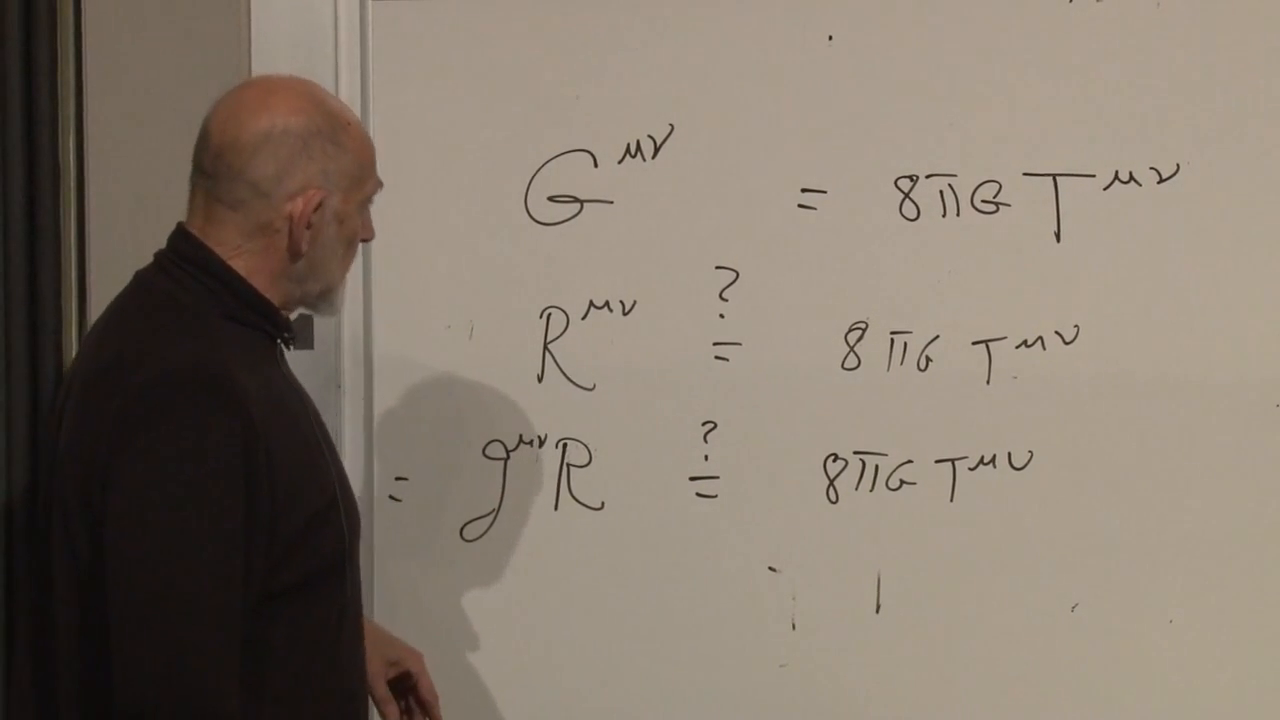
\includegraphics[width=0.78\textwidth]{lecture_09_figure_03.png}
\caption{Два пробных геометрических тензора на доске. На этом этапе оба имеют правильный ранг и правильный дифференциальный порядок, поэтому у каждого стоит вопросительный знак.}
\lectureframe{01:04:56}
\end{figure}

Рассматриваемые пробные варианты таковы
\begin{align}
 R_{\mu\nu}&\stackrel{?}{=}8\pi G\,T_{\mu\nu},\\
 g_{\mu\nu}R&\stackrel{?}{=}8\pi G\,T_{\mu\nu}.
\end{align}
Ни один нельзя принять лишь потому, что его индексы подходят. Проверку обеспечивает закон сохранения.

\section{Проверка дивергенцией}

Если верно уравнение~\eqref{eq:field-schematic}, то тождественно должно следовать
\begin{equation}
 D_\mu G^{\mu\nu}=0
\end{equation}
поскольку \(D_\mu T^{\mu\nu}=0\). Начнем с кандидата со скаляром кривизны. Правило произведения дает
\begin{equation}
 D_\mu\!\left(g^{\mu\nu}R\right)
 =
 \left(D_\mu g^{\mu\nu}\right)R
 +g^{\mu\nu}D_\mu R.
 \label{eq:product-rule}
\end{equation}

\begin{figure}[htbp]
\centering
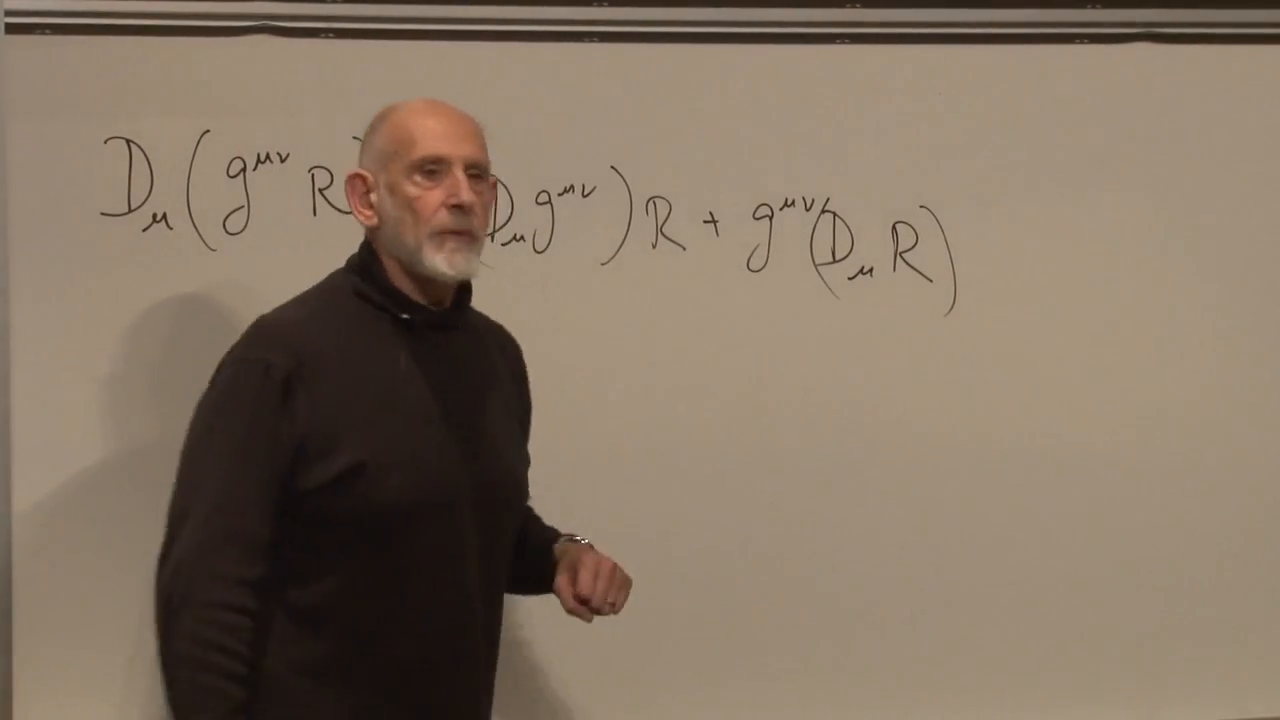
\includegraphics[width=0.84\textwidth]{lecture_09_figure_04.png}
\caption{Применение ковариантного правила произведения к
\(D_\mu(g^{\mu\nu}R)\).}
\lectureframe{01:07:12}
\end{figure}

Условие метрической совместимости гласит
\begin{equation}
 D_\mu g^{\alpha\beta}=0.
 \label{eq:metric-compatibility}
\end{equation}
Это независимое геометрическое свойство связности Леви-Чивиты, а не следствие сохранения энергии-импульса. Поскольку \(R\) — скаляр, \(D_\mu R=\partial_\mu R\). Поэтому уравнение~\eqref{eq:product-rule} принимает вид
\begin{equation}
 D_\mu(g^{\mu\nu}R)
 =g^{\mu\nu}\partial_\mu R
 =D^\nu R,
\end{equation}
что в общем случае не равно нулю. Кандидат \(g^{\mu\nu}R\) не проходит.

Соответствующее вычисление для тензора Риччи несколько длиннее. Его результатом является свернутое тождество Бьянки,
\begin{equation}
 D_\mu R^{\mu\nu}=\frac12 D^\nu R.
 \label{eq:contracted-bianchi}
\end{equation}
Следовательно, \(R^{\mu\nu}\) тоже само по себе не подходит. Но эти две неудачи находятся ровно в том отношении, которое нужно для взаимного сокращения:
\begin{equation}
 D_\mu\left(
 R^{\mu\nu}-\frac12 g^{\mu\nu}R
 \right)=0.
\end{equation}
Тем самым выбирается тензор Эйнштейна,
\begin{equation}
 \boxed{
 G_{\mu\nu}
 =
 R_{\mu\nu}-\frac12 g_{\mu\nu}R
 }.
 \label{eq:einstein-tensor}
\end{equation}

В рамках используемых здесь предположений -- о локальном симметричном тензоре второго ранга, построенном из метрики и содержащем не более двух производных, -- эта комбинация определяется с точностью до общего коэффициента и возможного метрического члена. Последний соответствует возможности космологической постоянной, к которой мы вернемся ближе к концу лекции. Коэффициент перед уравнением~\eqref{eq:einstein-tensor} фиксируется сопоставлением с ньютоновской гравитацией.

\begin{classroomqa}
\audiencequestion{Есть ли более прямой физический способ получить уравнение поля, а не перебирать кандидатов и отбрасывать их с помощью уравнения непрерывности?}
\lecturerresponse{Локальный закон сохранения уже является физическим принципом: энергия и импульс не могут исчезнуть из области, не пересекая ее границу. Есть и более сжатый вывод из принципа действия для гравитационного поля. Варьирование этого действия приводит к тому же уравнению, хотя само вычисление не короткое.
\lecturetimestamp{01:17:14--01:18:41}}
\end{classroomqa}

\begin{classroomqa}
\audiencequestion{Не мог бы какой-нибудь другой геометрический тензор второго ранга удовлетворять тому же закону сохранения? Является ли ответ физическим или математическим, и мог ли Эйнштейн это знать?}
\lecturerresponse{При предположениях этой конструкции классификация носит математический характер. Доступные объекты кривизны с двумя производными получаются из тензора Римана; два только что проверенных кандидата второго ранга исчерпывают соответствующие свертки. Для нахождения их комбинации с нулевой дивергенцией все равно требуется вычисление. Принципы просты, но труд заключается в обращении с индексами и знаками.
\lecturetimestamp{01:18:42--01:21:44}}
\end{classroomqa}

\section{Уравнение поля и его ньютоновский предел}

Уравнение поля теперь имеет вид
\begin{equation}
 \boxed{
 R_{\mu\nu}-\frac12 g_{\mu\nu}R
 =
 8\pi G\,T_{\mu\nu}
 }.
 \label{eq:einstein-equation}
\end{equation}
Левая часть геометрична; правая описывает материю, излучение и их потоки. Их ковариантные дивергенции обращаются в нуль совместно.

Множитель \(8\pi G\) не определяется аргументом с дивергенцией. Он определяется тем, что рассматривают слабое, медленно меняющееся гравитационное поле, порождаемое медленно движущейся материей, и требуют, чтобы временная-временная компонента воспроизводила уравнение Пуассона. В этом режиме \(T_{00}\simeq\rho\), тогда как остальные компоненты подавлены степенями \(v/c\). Геометрическая часть сводится к структуре со вторыми производными, предвосхищенной в уравнении~\eqref{eq:weak-mnemonic}. Сопоставление дает в точности нормировку в уравнении~\eqref{eq:einstein-equation}.

Этот предел также объясняет, почему ньютоновская гравитация кажется порождаемой только плотностью массы. В полной теории гравитирует каждая компонента \(T_{\mu\nu}\): плотность энергии, поток энергии, плотность импульса, давление и сдвиговые напряжения. Для обычной нерелятивистской материи доминирует энергия покоя. В релятивистской материи, излучении или системах с большим давлением остальными компонентами нельзя пренебрегать.

Исторический путь не был одной-единственной легкой догадкой. Тензор Риччи выглядит как очевидная первая попытка, а дополнительный член \(-\tfrac12g_{\mu\nu}R\) — именно то, что восстанавливает совместимость с локальным сохранением. Когда тензорная структура фиксирована, ньютоновский предел задает нормировку.

\section{Что остается после свертки}

\begin{classroomqa}
\audiencequestion{Когда четыре индекса тензора Римана сворачиваются до двух, имеет ли отброшенная информация физическое содержание?}
\lecturerresponse{Да. Тензор Риччи не содержит всей кривизны пространства-времени. Наиболее ясные примеры дают гравитационные поля без источников: тензор Риччи может обращаться в нуль, тогда как приливная кривизна и гравитационные волны сохраняются. Свертка сохраняет часть, непосредственно связанную с локальным уравнением источника, а не все степени свободы гравитационного поля.
\lecturetimestamp{01:21:57--01:23:10}}
\end{classroomqa}

Аналогия с электромагнетизмом полезна. Уравнения Максвелла допускают волны в области, не содержащей заряда или тока. Точно так же уравнение Эйнштейна допускает нетривиальную геометрию в области, где \(T_{\mu\nu}=0\). Теперь мы выведем более простое уравнение, которое там выполняется.

\section{Вакуум означает нулевой тензор Риччи, а не плоское пространство-время}

Положим
\begin{equation}
 T_{\mu\nu}=0.
\end{equation}
Тогда из уравнения~\eqref{eq:einstein-equation} получаем
\begin{equation}
 R_{\mu\nu}-\frac12g_{\mu\nu}R=0.
 \label{eq:vacuum-einstein}
\end{equation}
Свернём с \(g^{\mu\nu}\). Поскольку
\begin{equation}
 g^{\mu\nu}g_{\mu\nu}
 =\delta^\mu{}_\mu=4
\end{equation}
в четырёх измерениях пространства-времени, след равен
\begin{equation}
 R-\frac12(4)R=-R=0.
\end{equation}
Следовательно,
\begin{equation}
 R=0,
 \qquad
 R_{\mu\nu}=0.
 \label{eq:ricci-flat}
\end{equation}
Вакуумное полевое уравнение состоит в равенстве нулю тензора Риччи.

Крайне важно не заменять термин \emph{риччи-плоский} термином \emph{плоский}.
Внешняя область решения Шварцшильда не содержит вещества вне своей центральной сингулярности и удовлетворяет \(R_{\mu\nu}=0\). Однако её тензор Римана отличен от нуля, и приливные силы реальны. Можно проверить обращение тензора Риччи в нуль, вычислив вручную все символы Кристоффеля и компоненты кривизны, хотя это довольно утомительно, или предоставив рутинные выкладки системе символьной алгебры. В сингулярности классические выражения расходятся; всюду вне её вакуумное уравнение выполняется.

Гравитационные волны дают второй пример. Они могут распространяться в области без источников, неся при этом подлинное искривление пространства-времени. Таким образом,
\begin{equation}
 R_{\mu\nu}=0
 \quad\not\Rightarrow\quad
 R^\rho{}_{\sigma\mu\nu}=0.
\end{equation}

\section{Сохраняя источник: уравнение для следа}

Лекция почти завершается вакуумным результатом, но один из слушателей просит повторить свёртку, не отбрасывая источник.

\begin{classroomqa}
\audiencequestion{Что получится, если выполнить ту же свёртку, оставив \(T_{\mu\nu}\) в уравнении?}
\lecturerresponse{След напрямую связывает скалярную кривизну со следом тензора энергии-импульса, а подстановка этого соотношения обратно даёт эквивалентную форму полевого уравнения через тензор Риччи.
\lecturetimestamp{01:29:28--01:32:20}}
\end{classroomqa}

Определим
\begin{equation}
 T=g^{\mu\nu}T_{\mu\nu}.
\end{equation}
Взятие следа у уравнения~\eqref{eq:einstein-equation} даёт
\begin{align}
 R-\frac12(4)R&=8\pi G\,T,\\
 -R&=8\pi G\,T,
\end{align}
поэтому
\begin{equation}
 \boxed{R=-8\pi G\,T}.
 \label{eq:trace-relation}
\end{equation}
Подстановка обратно в полевое уравнение даёт
\begin{equation}
 \boxed{
 R_{\mu\nu}
 =
 8\pi G
 \left(
 T_{\mu\nu}-\frac12g_{\mu\nu}T
 \right)
 }.
 \label{eq:ricci-form}
\end{equation}

\begin{figure}[htbp]
\centering
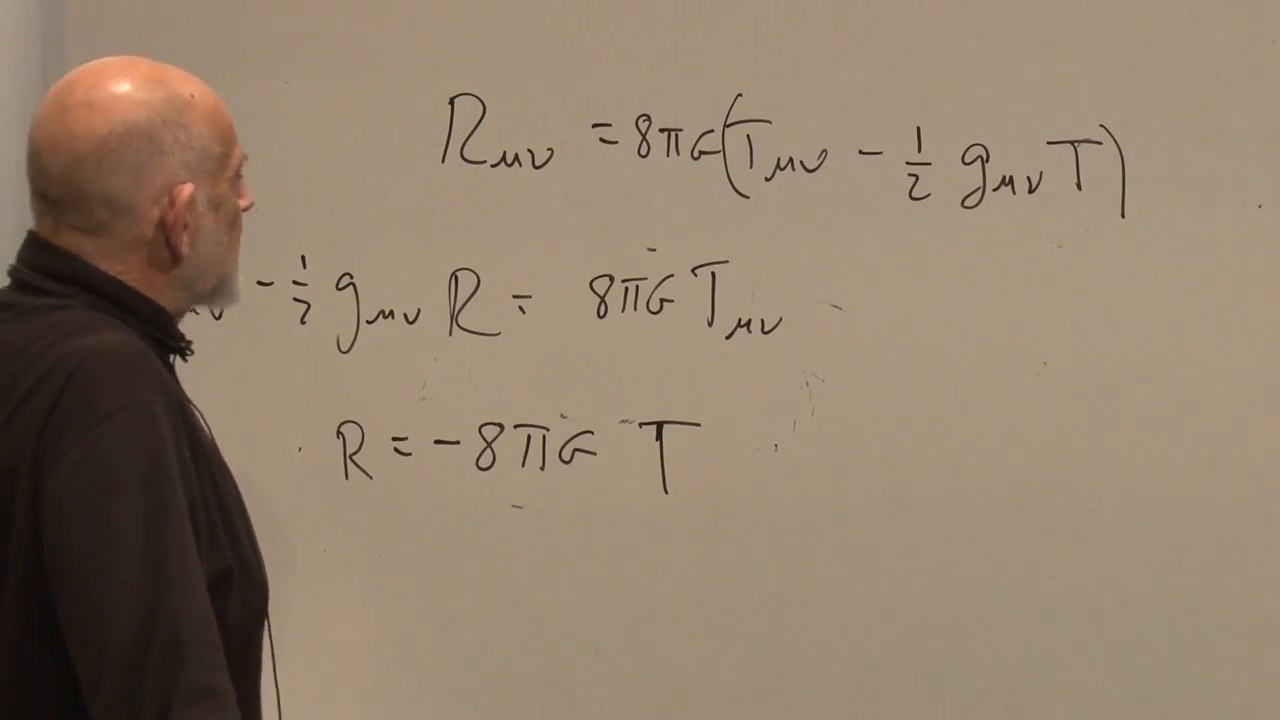
\includegraphics[width=0.82\textwidth]{lecture_09_figure_05.png}
\caption{Соотношение для следа и эквивалентная форма уравнения Эйнштейна через тензор Риччи.}
\lectureframe{01:32:25}
\end{figure}

\begin{classroomqa}
\audiencequestion{Имеет ли скаляр \(T\) физический смысл?}
\lecturerresponse{Это след тензора энергии-импульса. Для электромагнитного излучения он обращается в нуль, и то же верно для идеального газа безмассовых частиц, таких как фотоны. Для массивного вещества след, вообще говоря, отличен от нуля. Через уравнение~\eqref{eq:trace-relation} этот след определяет скалярную кривизну.
\lecturetimestamp{01:32:20--01:33:12}}
\end{classroomqa}

\section{Какую часть кривизны сохраняет тензор Риччи?}

\begin{classroomqa}
\audiencequestion{Есть ли простая физическая или геометрическая картина тензора Риччи и скаляра Риччи, сравнимая с параллельным переносом вокруг малого контура в случае тензора Римана?}
\lecturerresponse{Здесь не предлагается столь же наглядная картина. Тензор Римана непосредственно фиксирует поворот, возникающий при переносе вокруг малого контура. Его свёртки алгебраически проще, но их отдельные геометрические смыслы труднее наглядно представить. Лучше не выдумывать вводящую в заблуждение картину лишь потому, что она была бы удобна.
\lecturetimestamp{01:33:14--01:34:13}}
\end{classroomqa}

Количество информации, теряемой при свёртке, зависит от размерности. В четырёх измерениях тензор Римана содержит информацию о кривизне, отсутствующую в тензоре Риччи. В трёх измерениях тензор Римана определяется тензором Риччи. В двух измерениях скалярная кривизна содержит всю независимую информацию о кривизне. Поэтому в четырёхмерной гравитации есть место для степеней свободы кривизны без источников, невидимых для \(R_{\mu\nu}\).

\begin{classroomqa}
\audiencequestion{Если разные тензоры Римана могут иметь один и тот же тензор Риччи, то как эта недостающая информация проявляется физически?}
\lecturerresponse{Данный источник сам по себе не задаёт всякую возможную гравитационную конфигурацию. Граничные и начальные данные могут включать гравитационное излучение. В приближении слабого поля можно мыслить это так: начать с решения с источником и добавить свободную гравитационную волну. Полная нелинейная теория не допускает произвольной суперпозиции, но этот пример верно указывает на недостающую информацию: распространяющуюся кривизну, локально не фиксируемую \(T_{\mu\nu}\).
\lecturetimestamp{01:37:05--01:38:59}}
\end{classroomqa}

Теперь два вакуумных примера объединяются. Геометрия Шварцшильда несёт приливную кривизну вне массы. Гравитационная волна несёт свободно распространяющуюся кривизну. Каждый из этих случаев может удовлетворять \(R_{\mu\nu}=0\), оставаясь при этом неплоским.

\enlargethispage{1pt}
\section{Космологическая постоянная}

\begin{classroomqa}
\audiencequestion{Неужели нет никакого дополнительного подгоночного параметра, например космологической постоянной?}
\lecturerresponse{Космологическая постоянная допустима. Её можно записать в геометрической части как постоянную, умноженную на \(g_{\mu\nu}\), или перенести в правую часть и интерпретировать как вакуумный вклад в тензор энергии-импульса. Эти два описания — одно и то же уравнение при разном учёте членов.
\lecturetimestamp{01:39:01--01:40:44}}
\end{classroomqa}

При наличии космологической постоянной часто используют соглашение
\begin{equation}
 G_{\mu\nu}+\Lambda g_{\mu\nu}
 =
 8\pi G\,T_{\mu\nu}.
\end{equation}
Перенос дополнительного члена в правую часть определяет эффективный вакуумный тензор энергии-импульса,
\begin{equation}
 T_{\mu\nu}^{(\Lambda)}
 =
 -\frac{\Lambda}{8\pi G}g_{\mu\nu}.
\end{equation}
Поскольку метрическая совместимость даёт \(D_\mu g^{\mu\nu}=0\), дополнительный член автоматически совместим с законом сохранения. Это и есть метрический член, возможность которого оставляло открытой предыдущее утверждение о единственности.

\section{Меркурий и расчёт в приближении слабого поля}

\begin{classroomqa}
\audiencequestion{Пользовался ли Эйнштейн этим уравнением для расчёта орбиты Меркурия, и где можно увидеть, как был выполнен этот расчёт?}
\lecturerresponse{Эйнштейн работал ещё до того, как Шварцшильд получил точное решение, и вместо него использовал достаточно точное приближение для внешнего поля Солнца на больших расстояниях. Радиус Солнца и орбита Меркурия огромны по сравнению с радиусом Шварцшильда Солнца, поэтому релятивистские поправки малы. Он мог начать с кеплеровской орбиты и вычислить поправку по теории возмущений. Вскоре после этого Шварцшильд получил точное внешнее решение, сделав тот же расчёт систематическим.
\lecturetimestamp{01:40:46--01:43:48}}
\end{classroomqa}

Теория возмущений означает ровно это: начать с уже решённой задачи, а затем вычислить влияние малой поправки. Ньютонова сила, обратно пропорциональная квадрату расстояния, порождает замкнутые кеплеровы эллипсы. Общая теория относительности вносит небольшое отклонение в ньютоновское радиальное уравнение, поэтому эллипс не замыкается после одного оборота; его перигелий смещается.

Лекция завершается обсуждением любопытной исключительности замкнутых орбит в центральном поле. Сила обратных квадратов исключительна тем, что делает кеплеровы орбиты замкнутыми без прецессии. В более общем виде теорема Бертрана также выделяет потенциал изотропного гармонического осциллятора как другой центральный потенциал, при котором всякая связанная орбита замкнута. Малая релятивистская поправка снимает это ньютоново вырождение, превращая прецессию Меркурия в наблюдаемое проявление полевого уравнения, выведенного в этой главе.